\chapter{Algorytmy ewolucyjne}
\label{cha:genetyczne}

Algorytmami ewolucyjnymi nazywne są algoytmy, które w celu przeszukania przestrzeni rozwiązań  wykorzystują mechanizmy zaczerpnięte ze zjawiska ewolucji biologicznej. Jest to ogólna nazwa dla metod takich jak algorytmy genetyczne, strategie ewolucyjne czy neuroewolucje. 

Podobnie jak opisane w rozdziale \ref{cha:pso} algorytmy rojowe, ewolucyjne również zawierają populację agentów wpływających nawzajem na siebie. Populacja agentów generowana jest losowo, wraz z pewnym zestawem cech dla każdego agenta - genotypem. Genotyp jest takim zestawem cech agenta, który umiejscawia go w pewnej przestrzeni rozwiązań, co umożliwia jego ewaluację. Podczas działania algorytmu, agenci poprzez krzyżowanie się, umieranie i rodzenie wpływają na swoje genotypy. 

Na przestrzeni lat zostało zaproponowanych wiele algorytmów bazujących na mechanizmach genetycznych, jednak wszystkie z nich opierały się na tych samych bazowych mechanizmach. Każdy z osobników populacji mógł, zmieniając swój genotyp, przybliżyć całą populację do znalezienia optymalnego rozwiązania postawionego problemu. Większość wpółczesnych rozwiązań stosuje również krzyżowanie się osobników, jako drugą główną składową działania algorytmów tego typu.

\section{Przegląd wiedzy}
\label{sec:historiagenetycznych}
Początki algorytmów ewolucyjnych sięgają lat 50 XX wieku\cite{GA1}, jednak ich idee nie były rozwijane przez wiele lat, głównie ze względu na ograniczenia sprzętowe jak i metodologiczne. Dopiero dwadzieścia lat później\cite{GA2} pojawiły się prace rozwijające modele ewolucyjne. Wtedy też zostało zaproponowane twierdzenie Hollanda o schematach, które uważane jest za podstawę wyjaśnienia algorytmów genetycznych. 

Znaczącą kwestią wpływającą na tempo rozwoju algorytmów genetycznych, było użycie techniki uwzględniającej ewolucję zarówno przez mutację jak i krzyżowanie się osobników z danej populacji. Podczas kolejnych lat badań, algorytmy tego typu zostały poszerzone o kod genetyczny pozwalający reprezentować strukturę każdego problemu.

Klasyczne algorytmy ewolucyjne działają zgodnie z algorytmem przedstawionym na diagramie \ref{fig:GAdiagram}, lub podobnie do niego. 

\begin{figure}[H]
\begin{center} 
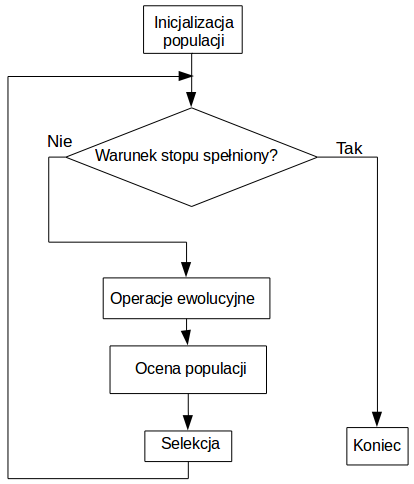
\includegraphics[scale=0.6]{tresc/pics/GAdiagram.png}
\caption{Diagram blokowy klasycznego algorytmu genetycznego}
\label{fig:GAdiagram}
\end{center}
\end{figure}

Początkowo inicjalizowana jest losowa populacja, która wykonuje między sobą zachowania ewolucyjne aż do spełnienia warunku stopu. Podczas każdej iteracji z całej populacji wybierana jest część osobników która zostanie poddana krzyżowaniu się między sobą. Następnie te osobniki poddawane są mutacji. Dla każdego z osobników wyliczana jest funkcja przystosowania, pozwalająca ocenić jakość jego genotypu.

\section{Algorytm EMAS}
https://github.com/ParaPhraseAGH/erlang-emas/wiki/EMAS-algorithm
https://age.iisg.agh.edu.pl/emas/intro.html

\subsection{Agent}

\subsection{Interakcje agentów}

\subsection{Ewolucja}

\subsection{Wyspy obliczeniowe}


\label{sec:emasOpis}









